
\section{Theorie}
\label{sec:Theorie}


 \subsection{Der photoelektrische Effekt und seine Erklärung mithilfe der Korspuskeltheorie  }


 \begin{figure}
 	\centering
 	\caption{Die Schaltung einer theoretischen Photodiode.}
 	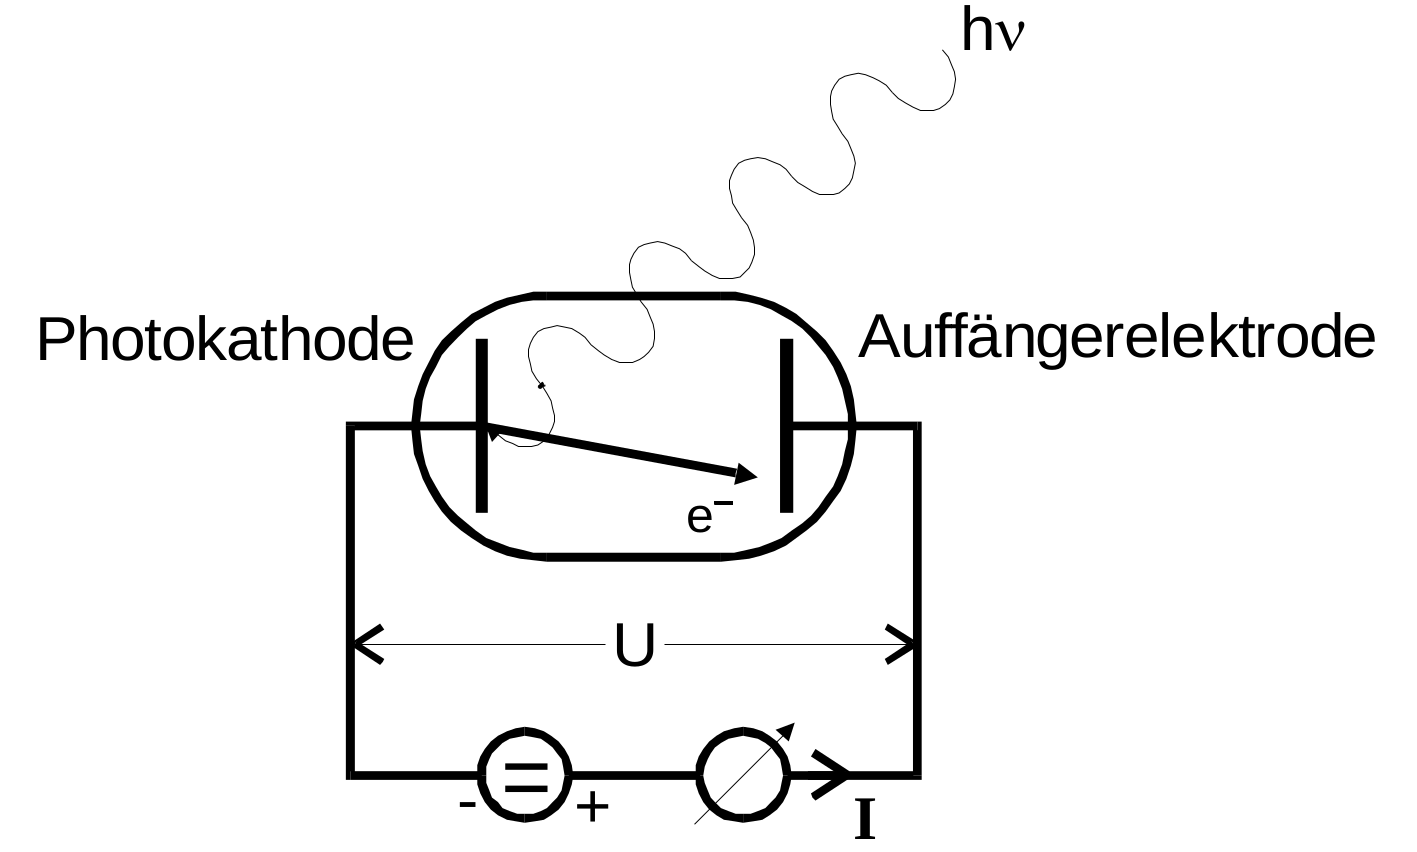
\includegraphics[width=\linewidth-170pt,height=\textheight-170pt,keepaspectratio]{content/Bilder/photodiode.png}
 	\label{fig:photodiode}
 \end{figure}


 Wird die Photokathode eines Photodiodenaufbaus wie in Abb. \cite{fig:photodiode}, welcher einer aus Kathodenrichtung
 beschleunigenden Spannnung mit monochromatischem licht bestrahlt kann ein Strom gemessen werden.
 Dieser Effekt wird lichtelektrischer Effekt gennant und weist mehrere Eigenschaften auf, welche mit dem
 klassischen Wellenbild des Lichtes nicht erklärt werden können.
\begin{itemize}
  \item Die Anzahl der aus dem Festkörper ausgelösten Elektronen verläuft
  proportional zur Intensität des Lichtes.
  \item die Energie der Photoelektronen ist unabhängig von der Intensität des
  Lichtes, verläuft jedoch proportional zu deren Frequenz.
  \item Unterhalb einer gewissen Lichtfrequenz $f_\text{g}$ tritt der Photoeffekt nicht auf
\end{itemize}
Alle Punkte lassen sich mit der Vorstellung erklären, dass das Licht aus einzelnen
Lichtteilchen den Photonen besteht. Sie entsprechen den Planckschen Energiequanten,
für welche gilt:
\begin{itemize}
  \item Monochromatisches Licht mit der Frequenz $f$ besteht aus Photonen,
  welche sich mit Lichtgeschwindigkeit bewegen und besitzen die Energie:
  \begin{equation}
    E = h \cdot f\text{.}\label{ITSAPLANCK}
    \end{equation}
    \item Trifft ein Photon auf ein Elektron überträgt es seine gesamte Energie.
    Ist diese größer als die benötigte Austrittsenergie $A_\text{k}$ verlässt
    dieses die Festkörperoberfläche mit der kinetischen Energie $E_\text{kin}$.
    Damit folgt:
    \begin{equation}
      h f = E_\text{kin} +A_\text{k}\text{.}\label{STEVE0ne:---3}
    \end{equation}
\end{itemize}
Zusätzlich besitzen die Elektronen jedoch bereits eine gewisse Energie. Die Wahrscheinlich,
mit welcher ein solches Energielevel auftritt wird über die Fermi-Dirac-verteilung
beschrieben. Deswegen kommt es bei der Grenzgegenspannung $U_\text{g}$ nicht zu
einem plötzlichen Einbruch der Stromstärke, sondern zu einem bereits vorher eintretenden abflachen.
